\documentclass{article}
\usepackage{import}
\subimport{../}{preamble}
\begin{document}

\section{Scanning Capacitive AFM Tip Alignment}
\label{sec:tip_alignment}

A significant challenge when attempting to recreate a plasmonic dimer using opposing AFM probes is the alignment of probes with the optical (laser) sampling spot in a symmetric tip-to-tip configuration. The ability to align two tips into a dimer configuration is necessary to enable the majority of dual tip experiments. This is the first step when measuring the dynamical physical response of such prototypical dimer systems.
For successful experiments the tolerance on the tip-to-tip alignment is less than \orderof{$R_{tip}$}. Aligning tips using CCD imaging in the microscope is limited by diffraction to around {\color{red}\SI{250}{nm}}. Initially this problem was solved using a non-linear capacitive alignment technique requiring locking into the third harmonic of the driving signal \cite{savage2011}. Whilst functional in simpler systems, the technique was limited in its accuracy due to small (\orderof{pA}) detectable currents in the third harmonic mode and the extensive filtering and lock-in techniques required to measure these. A simpler approach is to simply use the AFM module optics to measure the oscillating cantilever deflection. This is more widely known as scanning capacitance mode AFM (SC-AFM) or scanning capacitance microscopy (SCM). By utilising optical detection over direct electronic measurements tip alignment becomes segregated from the microscope electronic d.c. measurement circuitry and issues are no longer caused by noise leaking into the a.c. electronics.

% Scanning capacitance microscopy
SCM is a form of AFM used moreso in semiconductor doping analysis than in any other field \cite{huang1995quantitative}.

\subsection{Mechanism for Alignment of Two Opposing Tips}

\begin{figure}[h]
\centering
%\subimport{./figures/}{tip_alignment_diagram.tex}
\def\svgwidth{0.65\textwidth}
\subimport{./figures/}{tip_alignment_diagram.pdf_tex}
\caption[Diagram of tip alignment parameters]{\textbf{Diagram of tip alignment parameters.} The position of one tip relative to the other is detected using a resonant scanning capacitance AFM technique. The gap is biased with an oscillating voltage to induce a resonant vibration of one of the AFM cantilevers. The amplitude of oscillation is sensitive to the gap size $d$ and the area of overlap $A_{ov}$ between tip features of characteristic size $R$. For sharp tips $R$ is the apex radius whereas for nanostructured tips $R$ is considered to be the feature size.}
\label{fig:tip_alignment_diagram}
\end{figure}

% Describing the initial EoM of the full system
To a first approximation the metallic tips can be ignored and only the capacitive interaction between planar cantilevers is considered. Cantilevers are separated by a distance $d(t) = z_1(t) - z_2(t)$ and coupled via the $z$-components of the of the long range attractive electrostatic driving force $F_{EL}^z$ and short range (\orderof{nm}) Van da Waals and repulsive tip-tip interaction forces $F_{TT}^z$. Each cantilever has an associated spring constant $k_{0i}^z$, mass $m_i$ and resonant frequency of oscillation $\omega_{0i} = \sqrt{k_{0i}/m_i}$. When vibrated, cantilevers oscillate around an equilibrium position $z_{0i}$. The equilibrium separation between tips is then denoted by $d_0 = z_{01} - z_{02}$.

The equation describing motion in the $z$-axis of the two parallel cantilevers, denoted by $i=1,2$, of spring constant $k_i^z=k_{0i}^z+k_{TT}^z$, coefficient of damping $\beta_i^z=\beta_{0i}^z+\beta_{TT}^z$ and mass $m_i$, is given by,
\begin{equation}
m_i\frac{d^2z_i}{dt^2}+\beta_i^z\frac{dz_i}{dt}+k_i^z\left(z_i-z_{0i}\right)=\pm\left(F_{EL}^z+F_{TT}^z\right),
\end{equation}
where the sign of the force depends on the tip - positive for one tip and negative for the other.
% Simplifications
Assuming that alignment takes place at long range, tip-tip interactions can be ignored and $F_{TT}^z = 0$ and therefore $\beta_{TT}^{z} = k_{TT}^{z} = 0$. The system is further simplified by assuming that one cantilever remains stationary by being stiff (tapping mode $k\approx\SI{40}{N\per\metre}$) and always being off resonance ($\omega_{01} \neq \omega_{02}$). This is usually satisfied in experiments where a stiff cantilever is required such that the optical probe is incident on the same sample area whilst under force. The apex separation is then restricted to $d=z_1$ with an equilibrium separation $d_0 = z_{01}$. Under these conditions the motion reduces to that of a single tip,
\begin{equation}
m_1\frac{d^2z_1}{dt^2}+\beta_1^z\frac{dz_1}{dt}+k_1^z\left(z_1-d_0\right) = F_{EL}^z(z_1, t).
\label{eq:simple_eom}
\end{equation}
This equation now describes the whole system rather than each individual tip with the main reference point between tips being the equilibrium separation $d_0$.

% Description of the electrostatic force
The remaining capacitive driving force exerted between tips is purely electrostatic and of the form,
\begin{equation} F_{EL}^z(V,z) = \frac{1}{2} \frac{\partial C(z)}{\partial z} V^2(t), \end{equation}
where $C(z)$ is the capacitance between the tips at a distance $z$ and $V(t)$ is the potential difference between tips. Under a parallel plate capacitor model the capacitance is $C(z) = {\varepsilon_0 A_{ov}}/{z} + C_{bk}$ for plates with $A_{ov}$ area of overlap at a separation $z$, including a stray capacitance $C_{bk}$. Applying a harmonic driving force at a frequency $\omega_s$, $V(t)=V_0 \cos(\omega_s t)$, results in a nonlinear driving force, given by,
\begin{equation}
F_{EL}^z(z_1,t) = \left(\frac{-\varepsilon_0 A_{ov} V_0^2}{4z_1^2}\right)\left[1+\cos(\omega_pt)\right],
\label{eq:driving_force}
\end{equation}
where $\omega_p = 2\omega_s$ is the cantilever pump frequency.%
% Deriving the final EoM of the simplified system
Substituting \eqref{eq:driving_force} into \eqref{eq:simple_eom} gives the simplified equation of motion for the dual-tip system,
\begin{equation}
m_1 \frac{d^2z_1}{dt^2} + \beta_{01}^z \frac{dz_1}{dt} + k_{01}^z (z_1-d_0) = \left( \frac{-\varepsilon_0 A_{ov} V_0^2}{4z_1^2}\right)\left[1+\cos(\omega_pt)\right].
\label{eq:final_eom}
\end{equation}
Driving at a pump frequency close to the cantilever resonance ($\omega_p \approx \omega_{01}$) therefore leads to strong resonant oscillations between tips. For small oscillations around $d_0$ \eqref{eq:final_eom} can be solved approximately with a solution,
\begin{equation}
z_1 \approx d_0 - \left|z_{1}^{off}\right| - z_{m1}\cos(\omega_pt+\varphi_1)
\label{eq:tip_oscillation}
\end{equation}
where
\begin{subequations}
\begin{align}
z_1^{off} &\approx %
\frac{ \varepsilon_0 A_{ov} V_0^2 }{ 4d_0^2 \langle k_{e1}^z \rangle }, \label{eq:tip_amp}\\
%
z_{m1} &\approx %
\frac{ \varepsilon_0 A_{ov} V_0^2 }%
{ 4d_0^2 \sqrt{ (\langle k_{e1}^z \rangle - m_1\omega_p^2)^2 + (\beta_{01}^z\omega_p)^2  } }, \\
%
\varphi_1 &\approx \tan^{-1}\left(\frac{\beta_{01}^{z}\omega_{p}}{\langle k_{e1}^{z} \rangle -m_{1}\omega_{p}^{2}}\right), \label{eq:tip_phase}
\end{align}
\end{subequations}
in which $\langle k_{e1}^z \rangle$ is the effective spring constant of the system.

Although the model is for two parallel plates, it becomes applicable to tips in a dimer configuration once the separation is sufficiently low that the tip-to-tip capacitance dominates over all other capacitive contributions (such as the cantilever or tip facet interactions). Both the amplitude of the oscillations and the phase, given by \eqref{eq:tip_amp} and \eqref{eq:tip_phase}, depend on the tip-to-tip separation $d_0$. If the tips stray out of alignment the tip-to-tip distance increases and the capacitance, and by extension the tip oscillation, decreases, hence tips are aligned when the amplitude is maximised. Both properties sensitive to tip alignment can be readily measured using AFM cantilever deflection optics.

% Previous Electronic Alignment Methods without AFM Measurement
Whilst optical detection gives a better signal-to-noise and measures at higher bandwidths, it should be noted that the model was originally developed to show that the $3\omega_s$ current signal can be used to align tips \cite{savage2011}. By driving the system with $\omega_p \approx \omega_{01}$, a mechanical parametric resonance is excited at $2\omega_{01}$ (otherwise only the fundamental is excited with resonant driving) and the current through the tip junction is given by,
\begin{subequations}
\begin{align}
I(\omega_{s}) & \approx \omega_{s}C_{0}V_{0} \left(1+\frac{|z_{off}|}{d_{0}}+\frac{z_{m1}}{2d_{0}}e^{i\varphi_1}+\frac{C_{bk}}{C_{0}}\right)e^{i\frac{\pi}{2}},\\
%
I(\omega_{p}+\omega_{s}) & \approx \frac{\left(\omega_{p}+\omega_{s}\right)C_{0}V_{0}z_{m1}}{2d_{0}} e^{i\left(\varphi_1 + \frac{\pi}{2}\right)},
\label{eq:3rd_harmonic_current}
\end{align}
\end{subequations}
where $C_0 = \varepsilon_0 A^{ov} / d_0$ and $z_{off}$ is an additional offset due to $F_{EL}^z \propto V^2$. Non-linear oscillations in the tip capacitance result in parametric frequency mixing in the electronics with resulting signals at the sum and difference frequencies, $\omega_{p}+\omega_{s}=3\omega_{s}$ and $\omega_{p}-\omega_{s}=\omega_{s}$ respectively. The signal at $3\omega_{s}$ is background-free, as shown in \eqref{eq:3rd_harmonic_current}, and once again depends only on $z_{m1}$ and $d_{0}$. However, current are small (\orderof{pA}), therefore only alignment works over shorter ranges and requires larger voltages (for larger oscillation amplitudes) and low-noise detection electronics. Optical detection is advantageous as small oscillations at lower voltages are easily detectable, which protects the samples from damage caused by tip tapping when the gap is small.

\subsection{Numerical Solutions for Tip Alignment}

Theoretical curves for the system response based on \eqref{eq:final_eom} for a typically used contact/tapping mode AFM probe dimer are solved numerically using a ODE solver \footnote{ODE in Numpy/Python.}. Results are intended to \textit{qualitatively} demonstrate the alignment technique.
% Summary of parameters
The following table summarises the parameters of the model for each tip:
\begin{center}
\begin{tabular}{c | c | c}
\hline
& \textbf{Tip 1} & \textbf{Tip 2} \\
\hline                 
$k_0$ (N/m) & 0.2 & 40 \\
$\omega_0$ (kHz) & $2\pi.13$ & $2\pi.300$ \\
$\Delta\omega$ (Hz) & $2\pi.200$ & $2\pi.200$ \\
$r$ (nm) & 20 & 20 \\
\hline 
\end{tabular}
\end{center}
The plate area is assumed to be $\pi r^2$ where $r$ is the radius of the tip. This is estimated to be $r=\SI{20}{nm}$ based upon standard tip apex dimensions. Changing this value does not change the overall qualitative shape of the data. The mass of each tip is calculated from the resonance using $m_i = k_{0i}/\omega_{0i}^2$. The damping coefficient of each tip is given by $\beta_{0i} = 2m\delta_i$ where $\delta_i = \omega_{0i}/2Q_i$ and $Q_i = \omega_{0i}/\Delta\omega$. Only the camping coefficient of the vibrating tip matters at any given time due to the large difference in resonant frequencies. To maximise the detected response the system is studied around the resonance of the soft cantilever.
% The system model
The system spring constant is given by,
\begin{equation} k_0 = \left( k_{01}^{-1} + k_{02}^{-1} \right)^{-1}, \end{equation}
and the system mass is given similarly by,
\begin{equation} m = \left( m_1^{-1} + m_2^{-1} \right)^{-1}. \end{equation}
The damping coefficient of the system is calculated using,
\begin{equation}
\beta = 2m_1\delta_1 \left( 1 + \frac{r_1^2}{z} + \frac{(20e^{-6})^2}{z(2-20e^{-6})} \right),
\end{equation}
where $\delta = \Delta\omega/2$.

% Tip forces in the model
The forces acting on the tip are described by a capacitive driving force, described by \eqref{eq:driving_force}, and an interaction force. The interaction force is described by,
\begin{equation}
F_i^z(z) =
\begin{dcases}
-\frac{H r_1}{6(a+z_c)^2}, & \text{if } z_c + a > a_0 \\
-\frac{H r_1}{6a_0^2} + \frac{4E\sqrt{r_1}}{3 - 3v^2} (a_0-a-z_c)^{\frac{3}{2}}, & \text{otherwise}
\end{dcases}
\end{equation}
where $z_c$ is the equilibrium position, $a$ is the amplitude of the oscillation, $a_0$ is the equilibrium separation and $H$ is the Hamaker constant.
The capacitive driving force depends only upon the time-averaged tip separation whereas the interaction force depends on if the amplitude of the tip from its equilibrium separation causes contact/tapping with the other tip.

% Temporal response calculation
The ODE solving algorithm computes the change in the cantilever position and velocity in time using their respective differentials,
\begin{align}
\dot{z}_+ &= \dot{z}_-, \\
\ddot{z} &= -m^{-1}\left[\beta_1^z\dot{z} - k_0^zz + F_{EL}^z(t) + F_i^z(z)\right],
\end{align}
where $F_{EL}^z(t)$ is the capacitive driving force described in \eqref{eq:driving_force}, $F_i^z(z)$ is the interaction.
The response of the system in time to an applied force, subject to initial conditions, is solved for 100 AFM oscillation periods. The steady state harmonic properties of the waveform are then extracted using a sinusoidal fit to the last 50 periods. After 50 periods the system response has reached its steady state and is in most cases stable.

\begin{figure}[h]
\centering
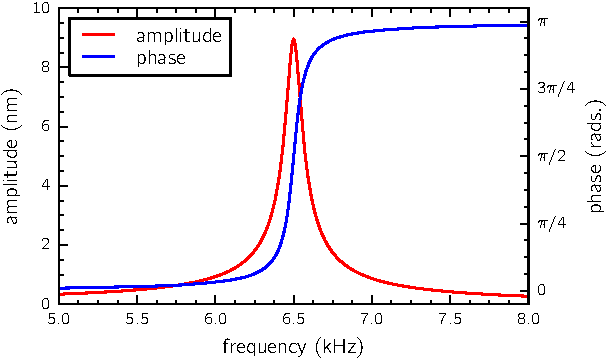
\includegraphics{figures/afm_theory_frequency_response}
\caption[Theoretical frequency response showing the amplitude and phase of a \SI{13}{kHz}-\SI{300}{kHz} opposing AFM tip system]{\textbf{Theoretical frequency response showing the amplitude and phase of a \SI{13}{kHz}-\SI{300}{kHz} opposing AFM tip system.} The tip junction is held at \SI{10}{V} with a \SI{100}{nm} intertip separation.}
\label{fig:num_freq_resp}
\end{figure}

% Frequency response
By driving a spatially fixed dimer system (tips separated by \SI{100}{nm} and biased with \SI{10}{V}) around $\omega_s = \omega_{01}/2 = 2\pi.\SI{13}{kHz}/2$ the frequency response of the tip dimer is determined and the tip resonance can be clearly seen. The intertip separation is then reduced while maintaining the resonant driving signal at $\omega_{01}/2$ to find the separation response.
\figurename~\ref{fig:num_freq_resp} shows the frequency response scanning through resonance. The line follows a Lorentzian line shape, typical of damped resonators, with a $\pi$ phase change when passing through resonance. The tip oscillates in phase with the second harmonic driving force below resonance and passes into anti-phase above resonance, in accordance with most resonators \cite{}.

\begin{figure}[h]
\centering
\fcapside[\FBwidth]
{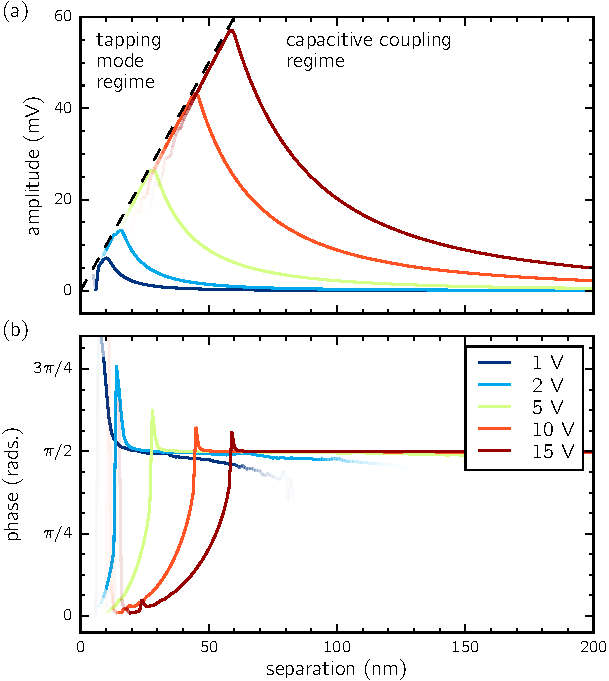
\includegraphics{figures/afm_theory_separation_response}}
{\caption[Theoretical separation response showing the amplitude (a) and phase (b) of a \SI{13}{kHz}-\SI{300}{kHz} opposing AFM tip system]{\textbf{Theoretical separation response showing the amplitude (a) and phase (b) of a \SI{13}{kHz}-\SI{300}{kHz} opposing AFM tip system.} The voltage across the tip junction is varied while on resonance ($\omega_s = 2\pi.\SI{6.5}{kHz}$). The amplitude increases as the intertip separation is reduced. The dashed line shows the point at which the oscillation amplitude is equal to the separation. For separations below this limit the hard surface restricts the amplitude to the gap between tips.}
\label{fig:num_sep_resp}}
\end{figure}

% Separation response
The separation response is shown in \figurename~\ref{fig:num_sep_resp}. As the separation decreases the capacitance between tips increases and the oscillation is amplified. This amplification occurs until the oscillation amplitude is equal to the separation, at which point the system transitions into the more regularly used tapping mode of AFM imaging. This is shown by the linear relationship between amplitude and separation regardless of voltage. In this regime the oscillation is restricted by the gap width between tips and so the separation limits the maximum possible amplitude.
Phase contrast only occurs once the oscillating tip can come into close proximity with the other tip. This degree of separation is confirmed by the onset of phase contrast being close to the point of maximum amplitude. The phase is therefore a good indicator of alignment between tips. Tips can be considered to be aligned once the amplitude and phase centres agree. The accuracy of these solutions becomes limited when the separation is reduced well into the tapping mode regime as the oscillation is difficult to sustain and surface (interfacial) forces begin to dominate leading to the snap-to-contact effect. This instability is seen by the deviation of the amplitude from its linear decrease in the tapping regime followed by its rapid decay.

\FloatBarrier
\subsection{Experimental Measurements using Scanning Capacitance Microscopy}

% Experimental acquisition
Experimental measurements of capacitive tapping mode tip interaction use the AFM optics on the microscope. The backside of the softer cantilever of the pair is illuminated by the \SI{633}{nm} laser beam from the AFM module. Reflected light from the cantilever is directed onto the position sensitive detector (PSD) where it generates a current depending on the location of the laser spot on the sensor.
By resonantly driving an AFM tip electronically its oscillation generates a signal $A\cos(\omega_p t + \phi)$ along one of the axes on the PSD. The current from the PSD is converted into an amplified voltage after padding through a signal processing circuit and transimpedance amplifier (\num{e5} gain). Lock-in detection is used to remove noise and add phase sensitivity to signal measurements by referencing the oscillation to the driving signal. Since the oscillation signal is large lock-in detection is performed using software rather than hardware, increasing the simplicity and reducing the overall cost of the setup. The NIDAQ device simultaneously acquires both the AFM PSD signals in each direction and the driving signal from the function generator output. The software lock-in detects the amplitude and phase of the tip oscillation by locking in on and isolating the second harmonic driving frequency $\omega_p$ using the reference periodicity. The phase difference $\phi$ is therefore measured between the signal and the reference.%
\footnote{The details of the lock-in procedure are detailed in the appendices.}

The resonance frequency of the {\color{red}(softer) back-facing} cantilever is determined prior to alignment by scanning the driving signal frequency and measuring the cantilever response. By mapping the lateral amplitude and phase variations of the cantilever deflection on resonance two opposing tips can be experimentally aligned. The location of the opposite tip is determined from the centroid of the mapped amplitude and phase variations. This procedure is advantageous as it operates at long range in the non-contact regime, prior to the tapping mode regime.

\begin{figure}[h]
\centering
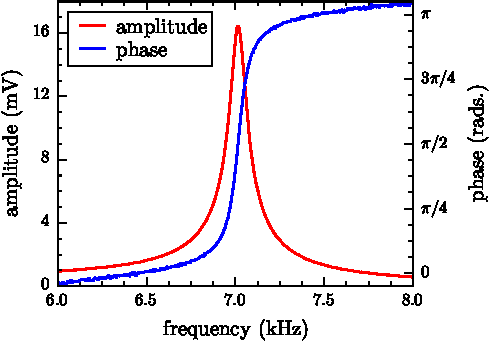
\includegraphics{figures/exp_resonance_scan}
\caption[Resonance scan of a standard Au contact mode AFM tip opposite a standard Au tapping mode AFM tip]{\textbf{Resonance scan of a standard Au contact mode AFM tip opposite a standard Au tapping mode AFM tip.} The soft tip (BudgetSensors ContGB) has a \SI{13}{kHz} resonant frequency and the stationary tip is resonant at \SI{190}{kHz} (BudgetSensors TapGB). Cantilevers are separated by $\sim$\SI{1}{\micro\metre} and driven at \SI{10}{V}.}
\label{fig:exp_freq_resp}
\end{figure}

The measured frequency response of a capacitively-driven AFM cantilever (\figurename~\ref{fig:exp_freq_resp}) agrees well with the modelled response (\figurename~\ref{fig:num_freq_resp}). One difference is the linear gradient superimposed onto the phase response. This stems from time lags during acquisition which give a linear phase offset with increasing frequency.

The separation response is probed by aligning a soft (\SI{13}{kHz}, \SI{0.2}{N\per\metre}) tip to the maximum amplitude signal by laterally scanning the $xy$ plane opposite a stiff (\SI{190}{kHz}, \SI{48}{N\per\metre}) tip. The soft tip is then approached towards the stationary tip along the $z$ axis in \orderof{nm} steps and the cantilever response is measured. The amplitude is monitored in real time and the tip is retracted once the signatures of tapping are detected and the regime is deemed to unstable to effects such as snap-in and short-range attractive forces or when there is a chance of damaging the tip. This judgement is subjective but preserves the tip for multiple cycles. This approach-reaction cycle is repeated many time with a continuously reducing voltage until tapping is difficult to achieve without immediately becoming unstable. This occurs once driving the oscillation with less than 5--\SI{6}{V}.

\begin{figure}[h]
\centering
\fcapside[\FBwidth]
{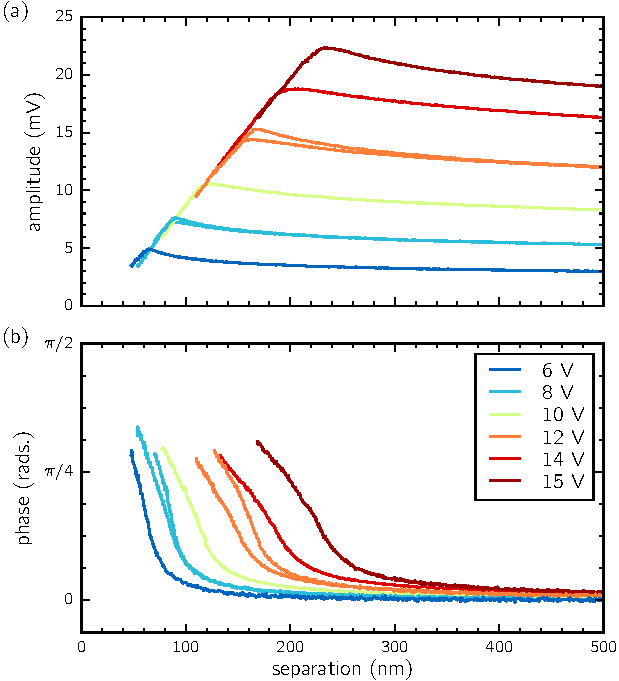
\includegraphics{figures/exp_separation_response}}
{\caption[Experimental separation response showing the amplitude (a) and phase (b) for a standard Au contact mode AFM tip approaching a standard Au tapping mode AFM tip]{\textbf{Experimental separation response showing the amplitude (a) and phase (b) for a standard Au contact mode AFM tip approaching a standard Au tapping mode AFM tip.} The same vibrating tip is approached and retracted with the voltage reduced between each approach cycle. The amplitude increases as the intertip separation is reduced until oscillation becomes restricted by the gap width.}
\label{fig:exp_sep_resp}}
\end{figure}

\figurename~\ref{fig:exp_sep_resp} shows the corresponding experimental curve to the numerically calculated separation response shown in \figurename~\ref{fig:num_sep_resp}. The expected capacitive increase in amplitude followed by a linear tapping mode regime is found in the experimental data. A significant difference from the model is that the baseline capacitive amplitude increase is not as drastic. This is likely due to the large extended shape of the tip. This was not taken account in numerical calculations which use only a simple parallel plate model. The linear decrease is also less steep suggesting that only the upper region of the modelled curve is visible.
The amplitude instabilities found in the theory for small separations and large driving amplitudes are also found in the experimental data. Repeat approaches after such an instability show different peak amplitudes with the differences attributed to misalignment after contact, changes in tip morphology or surface modification.
Interestingly the discontinuous reduction in the phase difference is not observed in the experiment. Either this means that a sufficiently restricted amplitude was not reached before retracting or that there is deviation from the simple model.
Overall the cantilever behaviour qualitatively matches many of the trends predicted using a simple mathematical model solved using an ODE solver.

\figurename~\ref{fig:exp_sep_resp} further demonstrates that this technique has the capability to lock the positions of the tips relative to each other at long range by using the graded separation response as a feedback mechanism. Dynamic positioning and alignment between two tips can then be locked and maintained through an experiment to account for fluctuations due to either mechanical or thermal drift. By using a \textit{pid} feedback loop and selecting a target amplitude the average position can be locked provided that the tip remains oscillating. By decreasing the voltage, oscillation can be reduced but only up until the point at which the second harmonic signal becomes difficult to detect. The onset of tapping also limits the minimum achievable separation though gap sizes well below \SI{100}{nm} remain possible. This technique could become more useful if a stable plasmonic gap size is required throughout an experiment whilst the contents or properties of the gap are modified.

\FloatBarrier
\subsection{Experimental Alignment of Tips using Scanning Capacitance AFM}

% The alignment procedure
Alignment between tips is carried out on resonance by laterally scanning the oscillating cantilever tip over the stationary, typically stiffer, tip whilst reducing the separation. To prevent tip collisions due to entering the tapping mode regime, the voltage is also reduced along with the separation. This allows only the minimum required signal for positional analysis. Unlike the phase, the amplitude signal varies smoothly over a longer range. By iteratively following the lateral position of maximum amplitude the tips can be brought into alignment. As the intertip separation decreases and the amplitude converges on this value the phase starts to increase forming a distinct, sharp peak around the tip apex.

\begin{figure}[h]
\centering
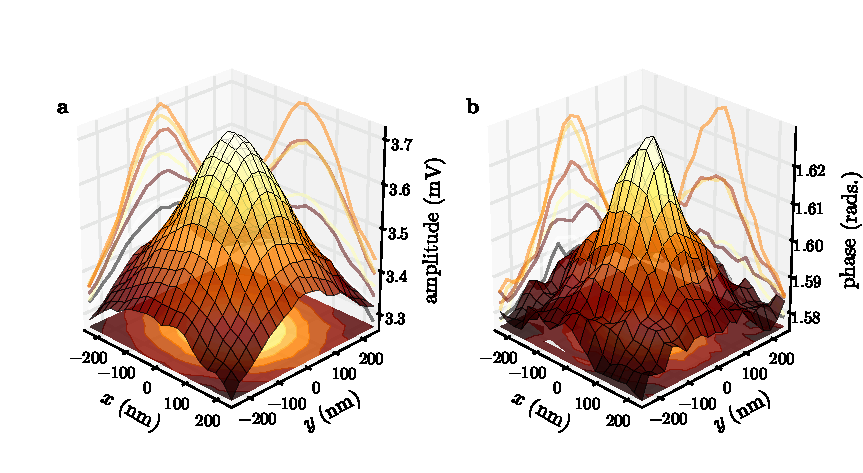
\includegraphics{figures/alignment_scan}
\caption[Alignment scan of a soft Au AFM tip scanned laterally over a hard Au AFM tip]{\textbf{Alignment scan of a soft Au AFM tip scanned laterally over a hard Au AFM tip.} The soft tip is oscillating at \SI{13}{kHz} (BudgetSensors ContGB) while the \SI{190}{kHz} Au tip (BudgetSensors TapGB) remains static. Tips are separated by $\sim$\SI{50}{nm} and driven at \SI{8}{V}. Strong peaks are seen in both the amplitude and the phase of the soft cantilever oscillation. The tips are aligned in a tip-to-tip configuration when both signals are maximised.}
\label{fig:alignment_scan} 
\end{figure}

\figurename~\ref{fig:alignment_scan} shows a typical alignment scan at close range with peaks in both the amplitude and phase when raster-scanning one tip over the other. At this point during the procedure the tips could be considered to be well aligned.

Since the tips are only symmetric in one direction capacitive coupling is {\color{red}inhomogeneous and skewed} until the distance between tips is small enough that the tip-to-tip capacitance dominates over the larger scale interactions. Gaussian fitting therefore can be potentially inaccurate in determining the peak location. Calculating the discrete image moments provides a more accurate, and faster, way of centring the scanned tip on the opposing tip. These are calculated using,
\begin{equation}
M_{ij} = \sum_x \sum_y x^i y^j I(x,y),
\end{equation}
where $i,j$ denote the possible axes \cite{}.%
\footnote{Note that the discrete image moments are based on the continuous moment theorem with moments given by $$M_{ij} = \int_{-\infty}^{\infty} \int_{-\infty}^{\infty} x^i y^j f(x,y) dx dy.$$}
The integrated intensity {\color{red}or area} of an image is given by the moment $M_{00} = \sum_x \sum_y I(x,y)$. The centroid of the image is then given by,
\begin{equation}
(\bar{x},\bar{y}) = \left( \frac{M_{10}}{M_{00}}, \frac{M_{01}}{M_{00}} \right).
\end{equation}
By tracking the centroid calculated at the end of each lateral scan whilst decreasing the tip separation from larger distances ($\sim$\SI{1}{\micro\metre}) to separations near to \SI{50}{nm} tips are brought into alignment.

\begin{figure}[h]
\centering
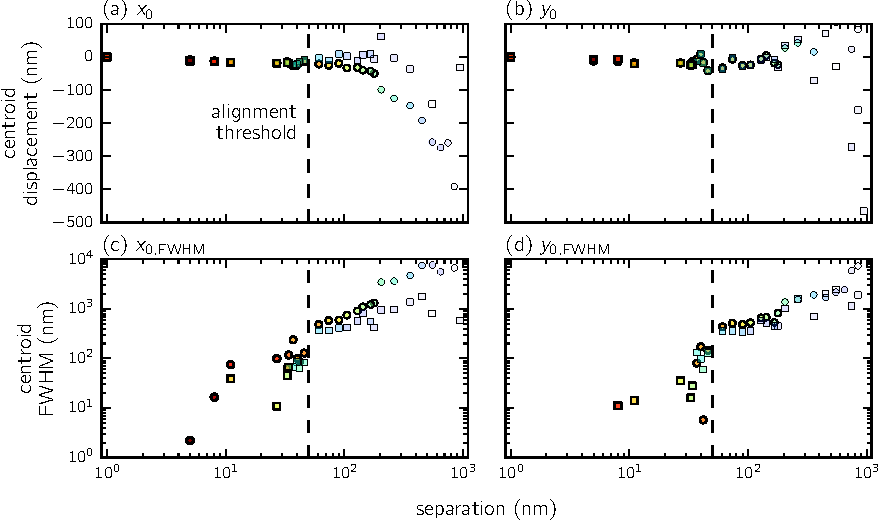
\includegraphics{figures/centroid_tracking}
\caption[Centroid tracking during approach and alignment of two sharp Au tips]{\textbf{Centroid tracking during approach and alignment of two sharp Au tips.} Amplitude (circles) and phase (squares) centroid positions relative to final alignment are shown in both the $x$ (a) and $y$ (b) directions. The centroid FWHM for the $x$ and $y$ amplitude and phase centroids are shown in (c) and (d), respectively. The final separation is an order of magnitude estimate based on the tapping mode linearity.}
\label{fig:centroid_tracking}
\end{figure}

Alignment is classified as the point at which the amplitude centroid is in agreement with the phase centroid. This criterion for alignment is chosen since the phase centroid does not deviate significantly from the initial position from which it emerges (\figurename~\ref{fig:centroid_tracking}(b)), despite only appearing once the separation has become sufficiently small. The amplitude centroid, on the other hand, follows the point of maximum capacitive coupling which depends sensitively on the separation regime and the driving voltage (\figurename~\ref{fig:centroid_tracking}(a)).
The accuracy of the alignment can be quantified from the FWHM of both the amplitude and phase peaks. The FWHM of both centroids shortly after passing the alignment threshold constrict to a similar length scale as the feature size dictating the short range alignment, such as the radius of a sharp or spherical tip apex. This level of localisation is directly visible in the data (\figurename~\ref{fig:centroid_tracking}(c,d)) where alignment using sharp Au tips results in a final FWHM between 10--\SI{30}{nm}. When studying spherical tips with \SI{150}{nm} radii it is noticed that the FWHM remains much larger since the surfaces in close proximity are much flatter in comparison. % Maybe need this graph for spherical tips but too costly to run?

%Alignment Capabilities and Limitations
The prerequisite requirements of this technique impose limitations as to which tip dimers can be formed. Tips necessarily have to be conductive to generate a strong capacitive signal at the tip junction and induce a cantilever resonance.%
\footnote{However it should be noted that Si tips have been aligned using this technique. Si AFM tips are generally doped to dissipate static charge. Here it is found that they are doped sufficiently to give an adequate capacitive response.}
Due to the increased sensitivity and signal-to-noise when using optical detection compared to electronics for long range alignment this technique is able to align together tips including those with smaller oscillations. This means that for a standard Au tip dimer (one contact, one tapping mode cantilever) alignment is possible at voltages as low as \SI{2}{V}, the minimum driving voltage of the input amplifier, for small tip separations. This means a lower current and a smaller oscillation amplitude, therefore less chance of damaging tips.

\begin{figure}[h]
\centering
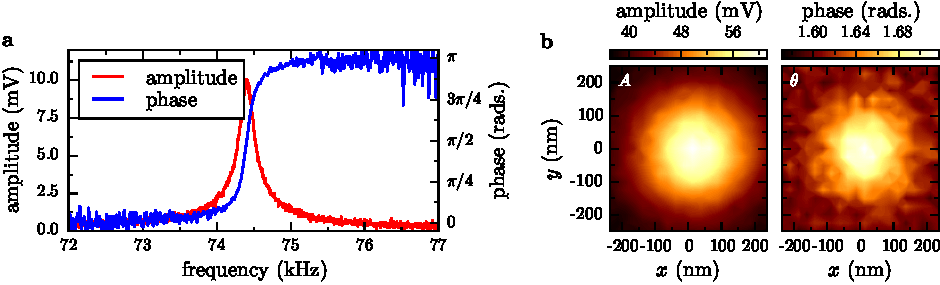
\includegraphics{figures/hf_alignment_data}
\caption[High frequency alignment data for a tip dimer composed of two \SI{48}{N\per\metre} Au AFM tips]{\textbf{High frequency alignment data for a tip dimer composed of two \SI{48}{N\per\metre} Au AFM tips.} Tips are separated by $\sim\SI{50}{nm}$ and driven at \SI{120}{V}. (a) Frequency response of the system. (b) Amplitude and phase alignment scans.}
\label{fig:hf_alignment_data} 
\end{figure}

Coupled with the higher bandwidth that the PSD offers (\SI{400}{kHz}) compared with sensitive electronics (\SI{100}{kHz}), this alignment technique has demonstrated the capability of aligning together pairs of cantilevers stiffer than the typically used contact mode probes. Cantilever resonances have been detected and alignment successfully performed for tip dimers comprised of $k=\SI{48}{N\per\metre}$ tapping mode (\SI{190}{kHz}) AFM probes (\figurename~\ref{fig:hf_alignment_data}), though in these cases the necessary driving voltage is increased to around \SI{100}{V}.

% Summary
To summarise, the capacitive alignment technique developed by Savage \textit{et al.} \cite{savage2011} has been successfully adapted to use optical cantilever detection, as in AFM, instead of direct electronic measurements of the tip junction. The technique is greatly improved, is less sensitive to other electronic systems integrated into the microscope, and has demonstrated the capability to align two tips to within \SI{10}{nm} of the target - less than the feature size of the tips. Both the frequency and spatial response is studied to show the tip separation dependence and the resulting alignment mechanism.

\end{document}